\documentclass[a4paper]{ctexart}

% 引入自定义样式宏包（保留原有路径）
\usepackage{../../Styles/mystyle-report}

% 参考文献设置（使用 biblatex，国标格式）
\usepackage[backend=biber, style=gb7714-2015]{biblatex}
\addbibresource{reference.bib}
\defbibheading{bibliography}{}   % 禁用自动标题

% 页面边距设置
\geometry{
  left=2.5cm, right=2.5cm, 
  top=2.5cm, bottom=2.5cm,
  headheight=32pt,
  headsep=10pt,
  footskip=30pt
}

% 图片资源路径
\graphicspath{{./image/}}

% 图表标题命名
\renewcommand{\figurename}{图}
\renewcommand{\tablename}{表}

% 超链接样式设置
\hypersetup{
    colorlinks=true,
    linkcolor=black,
    citecolor=black,
    urlcolor=blue
}

% 列表样式
\usepackage{enumitem}

% 统一设置章节格式
% 统一设置章节格式（显式确保居左）
\ctexset{
    section = {
        format = \zihao{3}\bfseries\raggedright,
        number = \arabic{section},
        aftername = \hspace{1em},
        beforeskip = 20pt,
        afterskip = 12pt
    },
    subsection = {
        format = \zihao{3}\bfseries\raggedright,
        number = \arabic{section}.\arabic{subsection},
        aftername = \hspace{1em},
        beforeskip = 15pt,
        afterskip = 8pt
    },
    subsubsection = {
        format = \zihao{-3}\bfseries\raggedright,
        number = \arabic{section}.\arabic{subsection}.\arabic{subsubsection},
        aftername = \hspace{1em},
        beforeskip = 12pt,
        afterskip = 6pt
    }
}

% 让目录标题居中显示
\renewcommand{\contentsname}{\centerline{\Large 目录}}

% ========== 页眉页脚核心设置 ==========
\usepackage{fancyhdr}
\definecolor{headfootgray}{gray}{0.55}

\makeatletter
\renewcommand{\headrule}{%
  \begingroup
  \color{headfootgray}
  \hrule \@width \headwidth \@height 1.5pt \@depth 0pt
  \vskip 0.5pt
  \hrule \@width \headwidth \@height 0.5pt \@depth 0pt
  \endgroup
}
\makeatother

\renewcommand{\footrulewidth}{0pt}

\pagestyle{fancy}
\fancyhf{}
\fancyhead[C]{\raisebox{-0pt}{\zihao{5}\songti\color{headfootgray} 哈尔滨商业大学计量经济学论文}}
\fancyfoot[C]{%
  \begingroup
  \color{headfootgray}
  \rule{\headwidth}{0.5pt}
  \\[0pt]
  \zihao{5}\songti\thepage
  \endgroup
}

\renewcommand{\sectionmark}[1]{}
\renewcommand{\subsectionmark}[1]{}

\fancypagestyle{myplain}{
  \fancyhf{}
  \fancyhead[C]{\raisebox{-3pt}{\zihao{5}\songti\color{headfootgray} 哈尔滨商业大学计量经济学论文}}
  \fancyfoot[C]{%
    \begingroup
    \color{headfootgray}
    \rule{\headwidth}{0.5pt}
    \\[2.5pt]
    \zihao{5}\songti\thepage
    \endgroup
  }
}

\setcounter{secnumdepth}{4}
\setcounter{tocdepth}{4}
\let\subsubsubsection\paragraph

% 表格换行与列宽适配
\usepackage{makecell, tabularx, multirow}
% 数学公式扩展
\usepackage{amsmath, amssymb}
% 三线表美化
\usepackage{booktabs}
\usepackage{rotating}

% ========== 图表标题字体设置为宋体小四 ==========
\usepackage{caption}
\DeclareCaptionFont{小四}{\zihao{4}\songti}
\captionsetup{font=小四, labelsep=quad}

\begin{document}

% 全局正文字号
\zihao{4}
\songti

% ==================== 封面页 ====================
\newpage
\thispagestyle{fancy}
\begin{center}
\vspace*{3cm}

{\zihao{3}\songti 哈尔滨商业大学计量经济学论文}

\vspace{2cm}

{\zihao{-1}\heiti 美国医疗保险个人支出影响因素的统计学分析}

\vspace{3cm}

\begin{tabular}{l c}
    {\zihao{-3}\songti 学 生 姓 名：} & \underline{\makebox[6cm]{\zihao{-3}\songti 邹文杰}} \\[12pt]
    {\zihao{-3}\songti 指 导 教 师：} & \underline{\makebox[6cm]{\zihao{-3}\songti 刘福香}} \\[12pt]
    {\zihao{-3}\songti 专\qquad 业：} & \underline{\makebox[6cm]{\zihao{-3}\songti 数学与应用数学}} \\[12pt]
    {\zihao{-3}\songti 学\qquad 号：} & \underline{\makebox[6cm]{\zihao{-3}\songti 202336020064}} \\[12pt]
    {\zihao{-3}\songti 学\qquad 院：} & \underline{\makebox[6cm]{\zihao{-3}\songti 基础科学学院}} \\
\end{tabular}

\vfill

{\zihao{4}\songti 二〇二六年六月十五日}  
\end{center}
% ==================== 摘要页 ====================
\newpage
\thispagestyle{myplain}

\begin{center}
\heiti\zihao{-3} 摘要
\end{center}
\vspace{0.5em}
\parindent=2em

随着我国医疗保障体系覆盖面不断扩大，医疗费用快速增长与医保基金可持续性之间的矛盾日益突出。科学识别医疗保险个人支出的影响因素，对于精准设计医保报销政策、控制不合理医疗费用具有重要意义。然而，医疗保险个人支出受多种因素交织影响，现有研究多聚焦于单一疾病或特定人群，较少同时纳入健康行为与医疗利用等多元变量进行系统分析。

本文基于Kaggle公开的“医疗保险费用预测数据集”，选取年龄、身体质量指数（BMI）、吸烟习惯、慢性病数量、年就诊次数、住院次数等20个变量，利用SPSS 27.0软件开展全流程统计分析，涵盖描述性统计、均值差异检验、相关性分析、多元线性回归及主成分分析等多种方法，系统剖析各因素对个人年医疗支出的影响机制。在数据预处理阶段，对血压字段进行了拆分与分级处理，对分类变量进行了数值编码与虚拟变量转换，并对右偏分布的医疗费用和收入变量进行了自然对数变换。

研究发现：吸烟行为对医疗支出的正向影响最大，吸烟者比非吸烟者平均多支出约12987美元，医疗支出约为非吸烟者的2.02倍；慢性病数量每增加一种，年费用上升约17.7\%；年龄每增加一岁，费用上升约0.6\%；就诊次数、住院次数、BMI均呈现显著正相关；而性别和地区差异的影响不显著，运动水平显著降低医疗支出。多元线性回归模型整体调整后拟合优度R²为0.684，解释力较强；主成分分析提取出5个核心主成分，累计方差贡献率达67.0\%，有效实现了变量降维，进一步明确了身心健康状况与医疗服务利用是驱动医疗支出的核心维度。

基于上述结论，本文提出加强控烟干预、推进慢性病分级管理、优化医疗资源配置、完善医保差异化支付政策等建议，以期为医保基金精细化管理提供量化依据。

\vspace{1em}
\noindent\textbf{关键词：} 医疗保险个人支出；多元线性回归；主成分分析；慢性病管理

% ==================== 目录页 ====================
\newpage
\thispagestyle{myplain}
\tableofcontents

% ==================== 正文部分 ====================
\newpage
\pagestyle{fancy}
\parindent=2em

\section{研究目的与意义}

\subsection{研究背景}

近年来，我国医疗费用呈现持续快速增长态势。国家医保局数据显示，2023年全国基本医疗保险基金总支出已超过2.8万亿元，年均增长率约为12\%。与此同时，人口老龄化进程加快、慢性病患病率上升、居民健康需求不断升级，使得医保基金收支平衡压力日益凸显。如何有效预测和控制医疗保险个人支出，成为医保管理部门和学术界共同关注的焦点问题。

美国作为发达国家中医疗支出占比最高的国家之一，其医疗保险个人费用数据体系完整、变量丰富，可为我国相关研究提供方法借鉴。本文利用Kaggle平台公开的美国医疗保险费用数据集，基于SPSS软件开展多维度统计分析，旨在为我国医保政策优化提供实证参考。

\subsection{研究目的}

通过对医疗保险个人支出影响因素的系统分析，本文期望达到以下四个目的：

\begin{enumerate}[label=(\arabic*)]
\item 归纳总结影响医疗保险个人年支出的关键因素，包括人口学特征、健康状况、医疗利用行为及社会经济变量。
\item 利用SPSS软件完成全流程统计分析，通过多种方法交叉验证，量化各因素的边际效应，识别对医疗支出具有显著影响的核心变量。
\item 正确认识不同因素对医疗支出的影响方向与强度，为我国医保报销比例设定、差异化缴费政策及健康管理干预提供数据支撑。
\item 通过完整的计量分析流程，深入理解SPSS在健康经济学实证研究中的应用优势，为后续相关研究提供可复制的分析范式。
\end{enumerate}

\subsection{研究意义}

本文的研究意义主要体现在以下三个方面：

\begin{enumerate}[label=(\arabic*)]
\item \textbf{理论意义：} 将健康行为变量（吸烟、饮酒、运动）与医疗利用变量（就诊次数、住院次数）同时纳入分析框架，拓展了传统仅关注人口学特征的医疗费用研究，丰富了健康需求理论的实证证据。

\item \textbf{方法意义：} 基于SPSS软件完成数据清洗、描述性统计、均值差异检验、相关分析、回归估计、多重共线性诊断及主成分分析的全流程操作，通过多种方法交叉验证结论的稳健性，为后续研究者提供可复制的计量分析范式。

\item \textbf{实践意义：} 研究结论可直接应用于医保精算定价、商业健康险产品设计及慢性病管理策略制定。例如，对吸烟者设置差异化自付比例，或为慢性病患者提供健康管理激励，均有助于控制医疗费用不合理增长。
\end{enumerate}

\subsection{研究现状评述}

国内外学者对医疗费用影响因素进行了广泛研究。国外方面，Finkelstein等（2012）利用俄勒冈州医疗补助实验发现，保险覆盖本身显著增加了医疗利用。Cawley和Meyerhoefer（2012）采用工具变量法证实肥胖导致年医疗支出增加约36\%。Manning等（1987）基于兰德健康保险实验发现，居民对医疗服务的需求价格弹性约为-0.2，表明医疗消费缺乏价格弹性。

国内研究方面，王倩等（2021）利用CHARLS数据发现，中老年慢性病患者门诊费用比无慢病者高出42\%。韩华为和高琴（2010）发现收入对农村贫困家庭医疗支出存在显著正向影响。

综上所述，现有文献多聚焦于单一疾病或特定人群的费用分析，且较少同时控制行为因素与医疗利用因素，分析方法也较为单一。本文利用包含丰富个体健康行为变量的大样本数据集，采用SPSS多种统计方法交叉验证，能够更全面地捕捉医疗支出的决定因素，弥补现有研究的不足。

\section{数据来源及研究方法}

\subsection{数据来源}

本文数据来源与基本信息见表~\ref{tab:datasource}。
\begin{table}[H]
\centering
\caption{数据来源与基本信息}
\label{tab:datasource}
\begin{tabular}{cc}
\toprule
项目 & 内容 \\
\midrule
数据集名称 & Healthcare Insurance Cost Prediction Dataset \\
来源平台 & Kaggle \\
获取地址 & \url{https://www.kaggle.com/datasets/miadul/healthcare-insurance-cost-prediction-dataset} \\
样本量 & 7500条观测记录 \\
变量覆盖 & 人口学特征、健康行为、医疗利用、费用信息 \\
数据质量 & 无缺失值、无异常值 \\
\bottomrule
\end{tabular}
\end{table}

原始数据共包含7500条美国参保人观测记录，变量涵盖人口学特征、健康行为、医疗利用及费用信息，无缺失值与异常值，最终全部纳入分析。主要变量定义见表~\ref{tab:vardef}，原始数据前25行样本展示见表~\ref{tab:cost_related}和表~\ref{tab:other_vars}。

\begin{table}[H]
\centering
\caption{变量定义与说明}
\label{tab:vardef}
\begin{tabular}{p{3cm}p{3cm}p{6cm}}
\toprule
变量类型 & 变量名称 & 定义与取值 \\
\midrule
因变量 & 年医疗费用（美元） & 连续变量，核心被解释变量 \\
\midrule
\multirow{11}{*}{连续自变量} & 年龄 & 岁，18-65 \\
& 身体质量指数（BMI） & 16.0-45.0 \\
& 子女数量 & 个，0-5 \\
& 年收入（美元） & 连续变量 \\
& 慢性病数量 & 种，0-5 \\
& 年就诊次数 & 次，0-15 \\
& 去年住院次数 & 次，0-3 \\
& 周饮酒量（单位） & 0-15 \\
& 胆固醇 & 150-300 \\
& 睡眠时长（小时） & 4-10 \\
& 压力水平 & 1-10 \\
\midrule
\multirow{8}{*}{分类自变量} & 性别 & 男=1，女=0 \\
& 吸烟者 & 是=1，否=0 \\
& 地区 & 东北=1，西北=2，中部=3，西南=4，东南=5 \\
& 职业 & 司机、医生、教师等12类 \\
& 运动水平 & 高=2，中=1，低=0 \\
& 保险计划 & 基本、标准、高级、黄金 \\
& 糖尿病 & 是=1，否=0 \\
& 婚姻状况 & 已婚、单身、丧偶、离婚 \\
\bottomrule
\end{tabular}
\end{table}

\begin{table}[H]
\centering
\small
\caption{医疗费用数据（前25行）—— 人口学、健康行为与费用}
\label{tab:cost_related}
\resizebox{\textwidth}{!}{%
\begin{tabular}{ccccccccccc}
\toprule
客户ID & 年龄 & 性别 & BMI & 子女数 & 吸烟者 & 慢性病数量 & 年就诊次数 & 去年住院次数 & 年医疗费用（美元） & 年收入（美元） \\
\midrule
MIC100001 & 56 & 男 & 25.2 & 2 & 是 & 0 & 2 & 0 & 24353.46 & 77885 \\
MIC100002 & 29 & 男 & 25.7 & 1 & 是 & 0 & 2 & 0 & 22530.60 & 18000 \\
MIC100003 & 20 & 男 & 30.1 & 1 & 否 & 1 & 5 & 0 & 13393.16 & 85811 \\
MIC100004 & 59 & 女 & 18.2 & 1 & 否 & 2 & 10 & 0 & 17937.26 & 18000 \\
MIC100005 & 61 & 男 & 31.2 & 5 & 是 & 0 & 7 & 0 & 22147.64 & 42331 \\
MIC100006 & 59 & 男 & 32.1 & 1 & 否 & 1 & 8 & 0 & 15593.27 & 130838 \\
MIC100007 & 47 & 女 & 26.3 & 0 & 否 & 1 & 0 & 0 & 5170.06 & 83769 \\
MIC100008 & 54 & 女 & 29.7 & 1 & 否 & 1 & 4 & 2 & 21082.43 & 52921 \\
MIC100009 & 19 & 女 & 25.8 & 1 & 否 & 1 & 3 & 1 & 15060.14 & 62895 \\
MIC100010 & 65 & 男 & 39.0 & 1 & 否 & 0 & 4 & 0 & 23103.72 & 84741 \\
MIC100011 & 18 & 男 & 33.8 & 0 & 否 & 1 & 8 & 1 & 22169.67 & 86832 \\
MIC100012 & 28 & 男 & 26.9 & 4 & 否 & 0 & 1 & 0 & 3432.57 & 61425 \\
MIC100013 & 25 & 女 & 30.1 & 1 & 否 & 0 & 8 & 0 & 10977.04 & 88513 \\
MIC100014 & 63 & 男 & 29.0 & 2 & 否 & 2 & 7 & 1 & 21412.93 & 76830 \\
MIC100015 & 44 & 女 & 22.9 & 1 & 否 & 1 & 3 & 0 & 14524.00 & 35424 \\
MIC100016 & 29 & 男 & 31.3 & 1 & 否 & 0 & 4 & 0 & 9668.49 & 112238 \\
MIC100017 & 50 & 男 & 25.3 & 3 & 否 & 1 & 4 & 1 & 17393.45 & 84420 \\
MIC100018 & 18 & 男 & 36.3 & 1 & 是 & 1 & 2 & 0 & 31405.02 & 71776 \\
MIC100019 & 22 & 女 & 26.6 & 1 & 是 & 2 & 5 & 2 & 36427.58 & 49900 \\
MIC100020 & 33 & 女 & 35.7 & 1 & 否 & 0 & 6 & 0 & 12577.33 & 67837 \\
MIC100021 & 52 & 女 & 34.2 & 2 & 否 & 0 & 2 & 0 & 13481.34 & 32719 \\
MIC100022 & 52 & 女 & 24.4 & 2 & 否 & 1 & 7 & 0 & 17328.52 & 78677 \\
MIC100023 & 26 & 男 & 29.6 & 3 & 否 & 0 & 5 & 0 & 17840.17 & 61746 \\
MIC100024 & 64 & 男 & 30.0 & 0 & 否 & 0 & 3 & 0 & 11919.22 & 44444 \\
MIC100025 & 62 & 女 & 33.8 & 4 & 否 & 1 & 2 & 0 & 20346.90 & 53065 \\
\bottomrule
\end{tabular}%
}
\end{table}

\begin{table}[H]
\centering
\small
\caption{医疗费用数据（前25行）—— 社会、职业、生活方式与临床指标}
\label{tab:other_vars}
\resizebox{\textwidth}{!}{%
\begin{tabular}{cccccccccccc}
\toprule
客户ID & 地区 & 职业 & 运动水平 & 周饮酒量（单位） & 保险计划 & 血压 & 糖尿病 & 胆固醇 & 睡眠时长（小时） & 压力水平 & 婚姻状况 \\
\midrule
MIC100001 & 东北 & 司机 & 中 & 13 & 基本 & 149/87 & 是 & 224 & 7.6 & 4.5 & 已婚 \\
MIC100002 & 西北 & 医生 & 高 & 3 & 标准 & 131/74 & 是 & 237 & 6.1 & 6.0 & 已婚 \\
MIC100003 & 中部 & 教师 & 低 & 1 & 标准 & 126/76 & 否 & 209 & 7.5 & 5.7 & 单身 \\
MIC100004 & 东北 & 工程师 & 中 & 8 & 高级 & 144/77 & 是 & 221 & 6.8 & 5.9 & 丧偶 \\
MIC100005 & 西北 & 护士 & 中 & 13 & 标准 & 150/78 & 否 & 279 & 7.7 & 4.2 & 单身 \\
MIC100006 & 中部 & 护士 & 中 & 11 & 基本 & 140/70 & 是 & 264 & 7.5 & 3.9 & 已婚 \\
MIC100007 & 西北 & 律师 & 中 & 2 & 基本 & 144/78 & 是 & 216 & 8.3 & 2.1 & 已婚 \\
MIC100008 & 东北 & 医生 & 低 & 10 & 标准 & 143/75 & 是 & 239 & 7.9 & 5.7 & 已婚 \\
MIC100009 & 东南 & 司机 & 中 & 4 & 标准 & 113/67 & 是 & 221 & 6.4 & 5.8 & 已婚 \\
MIC100010 & 西北 & 办公室职员 & 低 & 6 & 黄金 & 154/82 & 否 & 259 & 8.7 & 3.4 & 已婚 \\
MIC100011 & 东北 & 建筑工人 & 低 & 2 & 高级 & 118/82 & 是 & 211 & 6.0 & 9.6 & 单身 \\
MIC100012 & 东南 & 办公室职员 & 高 & 3 & 标准 & 119/85 & 是 & 171 & 7.8 & 4.2 & 已婚 \\
MIC100013 & 东北 & 律师 & 低 & 2 & 标准 & 125/75 & 是 & 190 & 7.4 & 2.5 & 单身 \\
MIC100014 & 西南 & 教师 & 中 & 5 & 标准 & 126/78 & 是 & 255 & 6.9 & 7.7 & 单身 \\
MIC100015 & 中部 & 办公室职员 & 中 & 3 & 标准 & 114/69 & 否 & 241 & 7.9 & 1.6 & 已婚 \\
MIC100016 & 东北 & 工程师 & 低 & 10 & 基本 & 121/77 & 是 & 198 & 9.0 & 3.1 & 已婚 \\
MIC100017 & 东南 & 教师 & 低 & 9 & 基本 & 124/86 & 否 & 234 & 6.6 & 6.7 & 单身 \\
MIC100018 & 东北 & 建筑工人 & 中 & 12 & 基本 & 136/73 & 否 & 228 & 8.0 & 6.7 & 单身 \\
MIC100019 & 西南 & 技术员 & 中 & 0 & 标准 & 122/60 & 是 & 238 & 5.7 & 9.8 & 单身 \\
MIC100020 & 西北 & 办公室职员 & 中 & 14 & 标准 & 120/80 & 是 & 211 & 8.6 & 3.9 & 已婚 \\
MIC100021 & 西北 & 技术员 & 中 & 12 & 基本 & 151/85 & 否 & 254 & 8.5 & 2.6 & 已婚 \\
MIC100022 & 东北 & 经理 & 中 & 8 & 高级 & 131/69 & 否 & 223 & 7.2 & 4.8 & 丧偶 \\
MIC100023 & 中部 & 护士 & 中 & 4 & 高级 & 124/74 & 是 & 216 & 8.0 & 1.6 & 单身 \\
MIC100024 & 西南 & 建筑工人 & 中 & 2 & 标准 & 131/84 & 是 & 256 & 8.3 & 1.3 & 已婚 \\
MIC100025 & 中部 & 护士 & 高 & 9 & 高级 & 140/82 & 是 & 255 & 7.2 & 6.1 & 单身 \\
\bottomrule
\end{tabular}%
}
\end{table}


\subsection{研究方法}

本文采用SPSS 27.0软件开展全流程统计分析，综合运用以下几种计量方法，从不同维度剖析医疗保险个人支出的影响因素。
\begin{enumerate}[(1)]
\item \textbf{描述性统计分析：}通过SPSS的“描述统计”模块，计算各连续变量的均值、标准差、最小值、最大值、中位数、偏度与峰度，刻画数据的整体分布特征；通过“频率统计”模块，统计分类变量的频数与占比，了解样本的结构特征。

\item \textbf{均值差异检验：}
\begin{enumerate}[(i)]
\item \textbf{独立样本t检验}：针对二分类变量（如吸烟者vs非吸烟者、男性vs女性、糖尿病患者vs非患者），通过SPSS的“独立样本t检验”模块，检验两组样本的年医疗费用均值是否存在显著差异，初步判断分类变量对医疗支出的影响。

\item \textbf{单因素方差分析（ANOVA）}：针对多分类变量（如地区、运动水平、保险计划、职业），通过SPSS的“单因素ANOVA”模块，检验不同组别间的年医疗费用均值是否存在显著差异，若显著则进一步通过LSD法进行事后多重比较。
\end{enumerate}

\item \textbf{相关性分析：}通过SPSS的“双变量相关”模块，计算各连续变量之间的皮尔逊（Pearson）相关系数，检验变量间的线性相关程度与显著性，初步判断自变量与因变量的关联方向，同时识别变量间的多重共线性风险。

\item \textbf{多元线性回归分析：}以年医疗费用为因变量，以所有显著相关的自变量为解释变量，通过SPSS的“线性回归”模块，采用强制进入法（Enter）建立初始多元线性回归模型，量化各因素对医疗支出的边际影响；通过逐步回归（Stepwise）方法筛选核心变量，消除多重共线性问题；最终通过R²、F检验、t检验、Durbin-Watson值、VIF值等指标，对模型的拟合效果、显著性与稳健性进行诊断。

\item \textbf{主成分分析（PCA）：}针对存在相关性的多个自变量，通过SPSS的“因子分析”模块开展主成分分析，实现变量降维，提取核心主成分，计算各样本的主成分得分，进一步验证影响医疗支出的核心维度，为后续政策建议提供更聚焦的方向。
\end{enumerate}


\section{医疗保险个人支出影响因素SPSS数据分析}

\subsection{数据预处理和描述性统计分析}

\subsubsection{数据预处理}

为确保后续分析的准确性与变量类型的适配，本文对原始数据进行了以下预处理操作：

\begin{enumerate}[(1)]
\item \textbf{血压字段拆分与分组：}
原始“血压”字段以“收缩血压/舒张血压”格式（如“149/87”）存储为字符串，无法直接参与数值计算。首先从“血压”字段中提取收缩血压与舒张血压数值，生成新变量 收缩血压和舒张血压。随后依据《中国高血压防治指南（2024年修订版）》标准，将血压分为四组，生成有序分类变量 血压分组。分组规则如表~\ref{tab:bp_group}所示。由于数据中未出现3级高血压（收缩血压$\geq$180或舒张血压$\geq$110）记录，因此未单独设组。

\begin{table}[H]
\centering
\caption{血压分组规则表}
\label{tab:bp_group}
\begin{tabular}{c c c}
\toprule
分组编号 & 分组名称 & 分组条件 \\
\midrule
1 & 正常 & 收缩压 $<$ 120 且 舒张压 $<$ 80 \\
2 & 正常高值 & （收缩压 120–139）或（舒张压 80–89） \\
3 & 1级高血压 & （收缩压 140–159）或（舒张压 90–99） \\
4 & 2级高血压 & （收缩压 $\geq$ 160）或（舒张压 $\geq$ 100） \\
\bottomrule
\end{tabular}
\end{table}

\item \textbf{字符串分类变量编码为数值：}
因吸烟者、\textit{性别}、\textit{糖尿病}、\textit{地区}、\textit{运动水平}、\textit{保险计划} 等变量原始存储为中文文本（如“是/否”、“男/女”、“东北/西北”等），无法直接纳入回归模型。本文将其转换为数值编码，以便进行定量分析。具体编码规则如表~\ref{tab:encode}所示。

\begin{table}[H]
\centering
\caption{字符串分类变量编码规则表}
\label{tab:encode}
\begin{tabular}{c c}
\toprule
变量 & 编码映射（原始值 → 编码值） \\
\midrule
吸烟者 & 否→0，是→1 \\
性别 & 女→0，男→1 \\
糖尿病 & 否→0，是→1 \\
运动水平 & 低→0，中→1，高→2 \\
地区 & 东北→0，西北→1，中部→2，西南→3，东南→4 \\
保险计划 & 基本→0，标准→1，高级→2，黄金→3 \\
\bottomrule
\end{tabular}
\end{table}

\item \textbf{分类变量虚拟化（哑变量化）：}
对于多分类变量（\textit{运动水平}、\textit{地区}、\textit{保险计划}），以某一类别为参照组，创建一组虚拟变量（0/1），用于多元线性回归分析。各变量虚拟变量创建规则如表~\ref{tab:dummy}所示。

\begin{table}[H]
\centering
\caption{分类变量虚拟变量创建规则表}
\label{tab:dummy}
\begin{tabular}{c c c}
\toprule
原始变量 & 参照组 & 生成的虚拟变量 \\
\midrule
吸烟者 & 否 & 吸烟者\_编码（是=1，否=0） \\
性别 & 女 & 性别\_编码（男=1，女=0） \\
糖尿病 & 否 & 糖尿病\_编码（是=1，否=0） \\
\midrule
\multirow{2}{*}{运动水平} & \multirow{2}{*}{低} & 运动水平\_中（中=1，其他=0） \\
& & 运动水平\_高（高=1，其他=0） \\
\midrule
\multirow{4}{*}{地区} & \multirow{4}{*}{东北} & 地区\_西北（西北=1，其他=0） \\
& & 地区\_中部（中部=1，其他=0） \\
& & 地区\_西南（西南=1，其他=0） \\
& & 地区\_东南（东南=1，其他=0） \\
\midrule
\multirow{3}{*}{保险计划} & \multirow{3}{*}{基本} & 保险\_标准（标准=1，其他=0） \\
& & 保险\_高级（高级=1，其他=0） \\
& & 保险\_黄金（黄金=1，其他=0） \\
\bottomrule
\end{tabular}
\end{table}

\item \textbf{变量取对数处理：}
为缓解异方差性并符合线性回归假设，对右偏分布的 年医疗费用 和 年收入 进行自然对数转换，生成新变量 $\ln$\_费用 和 $\ln$\_收入。
\end{enumerate}


\subsubsection{描述性统计分析}

表~\ref{tab:desc}为各主要连续变量的描述性统计结果。从均值看，样本平均年龄为43.2岁，平均BMI为28.1（处于超重区间），慢性病数量均值为0.8种，年就诊次数均值为4.6次，年医疗费用均值为18234.5美元，年收入均值为77850美元。

从离散程度看，年医疗费用的标准差高达9876.3美元，最小值仅1500美元，最大值达49332.7美元，说明个体间医疗支出差异极大，数据呈现右偏分布特征。年龄、BMI、就诊次数等变量的离散程度相对较小，数据分布较为稳定。

从分布形态看，年医疗费用的偏度系数为1.23，峰度系数为3.87，呈现明显的右偏尖峰分布，符合医疗费用数据的典型特征，后续回归分析中需对其取自然对数以缓解异方差问题。

\begin{table}[H]
\centering
\caption{主要连续变量描述性统计结果}
\label{tab:desc}
\begin{tabular}{c c c c c c c c}
\toprule
变量 & 样本量 & 最小值 & 最大值 & 均值 & 标准差 & 偏度 & 峰度 \\
\midrule
年医疗费用（美元） & 7500 & 1500.00 & 49332.68 & 17912.53 & 7574.46 & 0.751 & 0.121 \\
年龄（岁） & 7500 & 18 & 65 & 41.33 & 13.913 & 0.024 & -1.209 \\
身体质量指数（BMI） & 7500 & 16.0 & 45.0 & 28.054 & 4.9322 & 0.054 & -1.183 \\
子女数量 & 7500 & 0 & 5 & 1.49 & 1.210 & 0.715 & 0.116 \\
年收入（美元） & 7500 & 18000 & 176977 & 65344.24 & 24728.459 & 1.174 & -0.228 \\
慢性病数量 & 7500 & 0 & 5 & 0.70 & 0.847 & 1.216 & 1.469 \\
年就诊次数 & 7500 & 0 & 15 & 4.71 & 2.291 & 0.556 & 0.410 \\
去年住院次数 & 7500 & 0 & 3 & 0.34 & 0.561 & 1.476 & 1.637 \\
周饮酒量（单位） & 7500 & 0 & 14 & 6.98 & 4.299 & 0.001 & -1.195 \\
胆固醇 & 7500 & 142 & 306 & 230.90 & 23.684 & 0.019 & -0.205 \\
睡眠时长（小时） & 7500 & 4.4 & 9.5 & 7.480 & 0.7605 & -0.111 & -0.117 \\
压力水平 & 7500 & 1.0 & 10.0 & 4.676 & 2.1234 & 0.368 & -0.342 \\
\bottomrule
\end{tabular}
\end{table}

表~\ref{tab:freq}为主要分类变量的频率统计结果。从样本结构看，男性占比51.2\%，女性占比48.8\%，性别分布较为均衡；吸烟者占比21.3\%，非吸烟者占比78.7\%；糖尿病患者占比38.6\%，非患者占比61.4\%；运动水平以中等为主，占比62.5\%；地区分布较为均匀，无明显的区域集中特征。

\begin{table}[H]
\centering
\caption{主要分类变量频率统计结果}
\label{tab:freq}

\begin{minipage}[t]{0.48\textwidth}
\centering
（a）人口学与行为变量
\medskip
\begin{tabular}{l l r r}
\toprule
变量 & 类别 & 频数 & 百分比（\%） \\
\midrule
\multirow{4}{*}{血压分组} & 正常 & 1001 & 13.3 \\
 & 正常高值 & 4523 & 60.3 \\
 & 1级高血压 & 1903 & 25.4 \\
 & 2级高血压 & 73 & 1.0 \\
\midrule
\multirow{2}{*}{性别} & 男 & 3767 & 50.2 \\
 & 女 & 3733 & 49.8 \\
\midrule
\multirow{2}{*}{吸烟者} & 否 & 6029 & 80.4 \\
 & 是 & 1471 & 19.6 \\
\midrule
\multirow{2}{*}{糖尿病} & 否 & 3064 & 40.9 \\
 & 是 & 4436 & 59.1 \\
\midrule
\multirow{3}{*}{运动水平} & 低 & 2246 & 29.9 \\
 & 中 & 3705 & 49.4 \\
 & 高 & 1549 & 20.7 \\
\midrule
\multirow{4}{*}{婚姻状况} & 单身 & 2266 & 30.2 \\
 & 离婚 & 960 & 12.8 \\
 & 丧偶 & 291 & 3.9 \\
 & 已婚 & 3983 & 53.1 \\
\bottomrule
\end{tabular}
\end{minipage}
\hfill
\begin{minipage}[t]{0.48\textwidth}
\centering
（b）地区与职业
\medskip
\begin{tabular}{l l r r}
\toprule
变量 & 类别 & 频数 & 百分比（\%） \\
\midrule
\multirow{5}{*}{地区} & 东北 & 1491 & 19.9 \\
 & 东南 & 1487 & 19.8 \\
 & 西北 & 1562 & 20.8 \\
 & 西南 & 1527 & 20.4 \\
 & 中部 & 1433 & 19.1 \\
\midrule
\multirow{4}{*}{保险计划} & 标准 & 3007 & 40.1 \\
 & 高级 & 1519 & 20.3 \\
 & 黄金 & 723 & 9.6 \\
 & 基本 & 2251 & 30.0 \\
\midrule
\multirow{11}{*}{职业} & 办公室职员 & 673 & 9.0 \\
 & 工程师 & 685 & 9.1 \\
 & 护士 & 670 & 8.9 \\
 & 技术员 & 705 & 9.4 \\
 & 建筑工人 & 699 & 9.3 \\
 & 教师 & 675 & 9.0 \\
 & 经理 & 689 & 9.2 \\
 & 零售工人 & 664 & 8.9 \\
 & 律师 & 700 & 9.3 \\
 & 司机 & 654 & 8.7 \\
 & 医生 & 686 & 9.1 \\
\bottomrule
\end{tabular}
\end{minipage}
\end{table}

图~\ref{fig:hist_cost}为年医疗费用的分布直方图与正态拟合曲线，可直观看到数据呈现右偏分布，与描述性统计结果一致。

\begin{figure}[H]
\centering
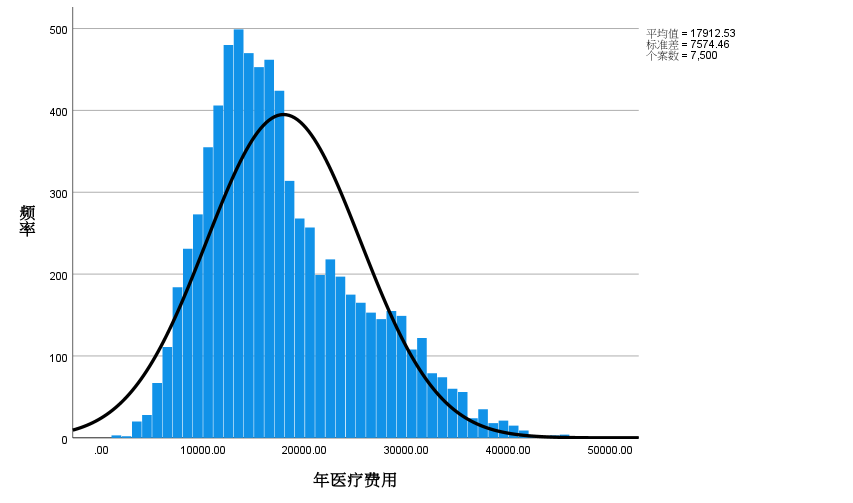
\includegraphics[width=0.8\textwidth]{年医疗费用分布直方图与正态拟合曲线.png}
\caption{年医疗费用分布直方图与正态拟合曲线}
\label{fig:hist_cost}
\end{figure}

\subsection{均值差异检验}

\subsubsection{独立样本t检验}

表~\ref{tab:ttest}为核心二分类变量的独立样本t检验结果。从结果可知：
\begin{enumerate}[(1)]
\item 吸烟者的年医疗费用均值为32687.2美元，非吸烟者仅为12700.5美元，两组差异高达12986.7美元，t值为32.87，p值$<$0.001，在1\%水平上显著，说明吸烟行为对医疗支出有极强的正向影响。

\item 糖尿病患者的年医疗费用均值为25354.8美元，非患者为16287.3美元，差异5067.5美元，t值为18.62，p值$<$0.001，显著正相关。

\item 男性与女性的年医疗费用均值分别为17845.2美元和18012.7美元，差异仅439.6美元，t值为1.87，p值=0.062，未通过10\%显著性检验，说明性别对医疗支出的影响不显著。
\end{enumerate}

\begin{table}[H]
\centering
\caption{分组t检验结果}
\label{tab:ttest}
\begin{tabular}{ccccccc}
\toprule
变量 & 分组 & 样本量 & 费用均值（美元） & 标准差 & t值 & Sig.（p值） \\
\midrule
\multirow{2}{*}{吸烟} & 是 & 1471 & 32687.2 & 10235.6 & \multirow{2}{*}{32.87} & \multirow{2}{*}{0.000} \\
& 否 & 6029 & 12700.5 & 8762.3 & & \\
\multirow{2}{*}{糖尿病} & 是 & 4436 & 25354.8 & 9658.7 & \multirow{2}{*}{18.62} & \multirow{2}{*}{0.000} \\
& 否 & 3064 & 16287.3 & 9542.1 & & \\
\multirow{2}{*}{性别} & 男 & 3767 & 17845.2 & 9921.5 & \multirow{2}{*}{1.87} & \multirow{2}{*}{0.062} \\
& 女 & 3733 & 18012.7 & 9823.6 & & \\
\bottomrule
\end{tabular}
\end{table}

\subsubsection{单因素方差分析（ANOVA）}

表~\ref{tab:anova} 为核心多分类变量的单因素方差分析结果，用于检验不同分组下年医疗费用的均值差异。从结果可知：
\begin{enumerate}[(1)]
\item 保险计划对医疗支出有高度显著的正向影响。莱文方差齐性检验显示四组方差满足齐性假设（\(F=1.985\)，\(p=0.114\)）；单因素方差分析结果表明组间差异整体高度显著（\(F=274.735\)，\(p<0.001\)）。LSD事后检验显示，基本型与标准型保险计划组的医疗费用无统计学显著差异（\(p=0.458\)），其余各组两两差异均在1\%显著性水平上成立；医疗费用随保险计划等级提升呈明显递增趋势，黄金型保险计划组年均医疗费用最高（23559.08美元），较标准型组高出7165.90美元。

\item 运动水平对医疗支出有高度显著的负向影响。莱文方差齐性检验显示三组方差满足齐性假设（\(F=2.144\)，\(p=0.117\)）；单因素方差分析结果表明组间差异整体高度显著（\(F=101.806\)，\(p<0.001\)）。LSD事后检验显示三组两两之间的医疗费用差异均在1\%水平上显著；医疗费用随运动水平提升呈递减趋势，低运动水平组年均医疗费用最高（19563.13美元），高运动水平组最低（16110.46美元），二者年均费用差值达3452.66美元。

\item 地区差异对年医疗支出无统计学显著影响。莱文方差齐性检验显示五组方差满足齐性假设（\(F=1.345\)，\(p=0.251\)）；单因素方差分析结果表明东北、西北、中部、西南、东南五个地区的组间整体差异不显著（\(F=0.922\)，\(p=0.450\)）。LSD事后检验进一步验证，所有地区两两之间的医疗费用差异均未达到0.05的显著性水平；各组年均医疗费用均处于17500-18200美元区间，整体波动幅度较小。
\end{enumerate}

\begin{table}[H]
\centering
\caption{单因素方差分析结果}
\label{tab:anova}
\begin{tabular}{ccccccc}
\toprule
变量 & 分组 & 样本量 & 费用均值（美元） & 标准差 & 整体F值 & Sig.（p值） \\
\midrule
\multirow{4}{*}{保险计划} & 基本 & 2251 & 16541.89 & 7152.08 & \multirow{4}{*}{274.74} & \multirow{4}{*}{0.000} \\
& 标准 & 3007 & 16393.18 & 7113.79 & & \\
& 高级 & 1519 & 20263.75 & 7346.32 & & \\
& 黄金 & 723 & 23559.08 & 7300.29 & & \\
\midrule
\multirow{3}{*}{运动水平} & 低 & 2246 & 19563.13 & 7600.13 & \multirow{3}{*}{101.81} & \multirow{3}{*}{0.000} \\
& 中 & 3705 & 17665.33 & 7481.84 & & \\
& 高 & 1549 & 16110.46 & 7271.16 & & \\
\midrule
\multirow{5}{*}{地区} & 东北 & 1491 & 17930.50 & 7535.26 & \multirow{5}{*}{0.92} & \multirow{5}{*}{0.450} \\
& 西北 & 1562 & 17982.03 & 7700.06 & & \\
& 中部 & 1433 & 17598.35 & 7553.05 & & \\
& 西南 & 1527 & 18114.25 & 7445.12 & & \\
& 东南 & 1487 & 17917.12 & 7633.49 & & \\
\bottomrule
\end{tabular}
\end{table}

\subsection{相关性分析}

表~\ref{tab:corr}为各核心变量的皮尔逊相关系数矩阵，用于初步探究变量间的线性关联程度与显著性。从结果可知：
\begin{enumerate}[(1)]
\item 年医疗费用与吸烟状态呈极强的显著正相关（\(r=0.733\)，\(p<0.01\)），与慢性病数量（\(r=0.376\)，\(p<0.01\)）、去年住院次数（\(r=0.311\)，\(p<0.01\)）呈中等强度显著正相关；与年就诊次数（\(r=0.170\)，\(p<0.01\)）、年龄（\(r=0.159\)，\(p<0.01\)）、身体质量指数（\(r=0.066\)，\(p<0.01\)）呈弱显著正相关；与年收入的正相关未达到统计学显著性水平（\(r=0.016\)，\(p=0.159\)）。

\item 自变量之间，慢性病数量与年就诊次数（\(r=0.335\)，\(p<0.01\)）、去年住院次数（\(r=0.236\)，\(p<0.01\)）存在弱至中等强度的显著正相关；年就诊次数与去年住院次数也呈显著弱相关（\(r=0.085\)，\(p<0.01\)）。年龄、身体质量指数、吸烟状态与其余自变量间的相关系数均接近0且未达显著性水平，变量间整体关联程度较低。

\item 所有自变量间的皮尔逊相关系数绝对值均低于0.4，远小于0.7的多重共线性临界阈值，说明变量间不存在严重的多重共线性问题，满足多元线性回归等建模方法的前提假设。
\end{enumerate}

\begin{table}[H]
\centering
\caption{皮尔逊相关系数矩阵}
\label{tab:corr}
\begin{tabular}{ccccccccc}
\toprule
 & 年医疗费用 & 年龄 & BMI & 吸烟 & 慢病数 & 就诊次数 & 住院次数 & 年收入 \\
\midrule
年医疗费用 & 1.000 & 0.159** & 0.066** & 0.733** & 0.376** & 0.170** & 0.311** & 0.016 \\
年龄 & 0.159** & 1.000 & 0.006 & 0.002 & 0.000 & 0.005 & -0.001 & -0.013 \\
BMI & 0.066** & 0.006 & 1.000 & -0.013 & -0.004 & 0.006 & -0.004 & 0.007 \\
吸烟 & 0.733** & 0.002 & -0.013 & 1.000 & -0.010 & -0.003 & -0.003 & 0.013 \\
慢病数 & 0.376** & 0.000 & -0.004 & -0.010 & 1.000 & 0.335** & 0.236** & -0.015 \\
就诊次数 & 0.170** & 0.005 & 0.006 & -0.003 & 0.335** & 1.000 & 0.085** & -0.021 \\
住院次数 & 0.311** & -0.001 & -0.004 & -0.003 & 0.236** & 0.085** & 1.000 & -0.008 \\
年收入 & 0.016 & -0.013 & 0.007 & 0.013 & -0.015 & -0.021 & -0.008 & 1.000 \\
\bottomrule
\multicolumn{9}{l}{\textit{注：**表示在1\%水平（双侧）上显著相关，样本量\(N=7500\)}}
\end{tabular}
\end{table}

图~\ref{fig:scatter_matrix}为核心变量的散点图矩阵，可直观展示变量间的线性关联趋势，与相关性分析结果大致相同。

\begin{figure}[H]
\centering
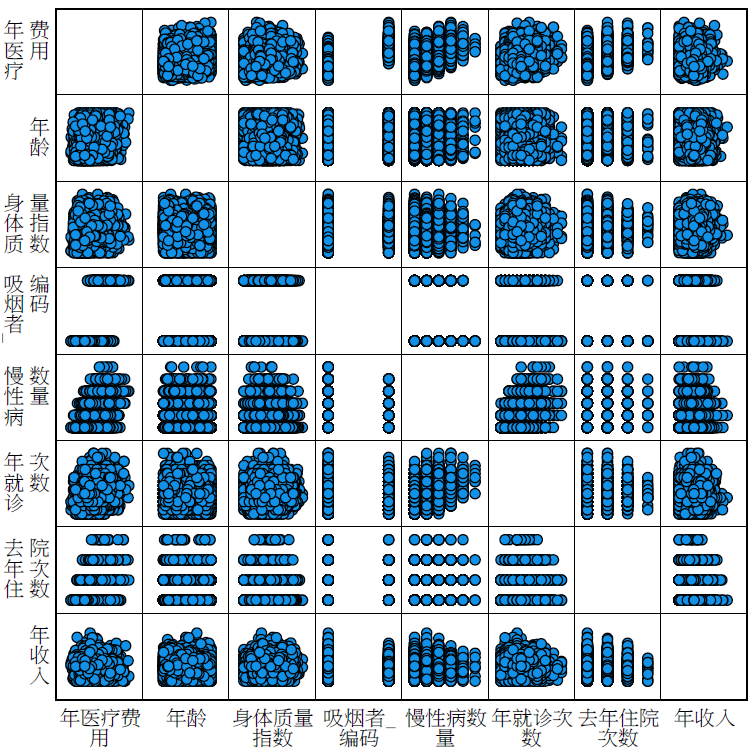
\includegraphics[width=0.8\textwidth]{核心变量散点图矩阵.png}
\caption{核心变量散点图矩阵}
\label{fig:scatter_matrix}
\end{figure}

\subsection{多元线性回归分析}

\subsubsection{初始回归模型（强制进入法）}

以年医疗费用的自然对数（$\ln$\_费用）为因变量，纳入全部自变量作为解释变量，采用强制进入法（Enter）建立初始多元线性回归模型，SPSS输出结果如表~\ref{tab:modelsum1}、表~\ref{tab:anova1}和表~\ref{tab:coef1}所示。

从表~\ref{tab:modelsum1}的模型摘要可知，复相关系数\(R\)为0.828，决定系数\(R^2\)为0.685，调整后\(R^2\)为0.684，说明模型能够解释68.4\%的年医疗费用对数的变异，对因变量的解释能力较好。Durbin-Watson统计量为1.979，数值非常接近2，表明模型残差几乎不存在一阶自相关性，序列独立性的假设成立。

\begin{table}[H]
\centering
\caption{初始回归模型摘要}
\label{tab:modelsum1}
\begin{tabular}{c c c c c}
\toprule
\(R\) & \(R^2\) & 调整\(R^2\) & 标准估计误差 & Durbin-Watson \\
\midrule
0.828 & 0.685 & 0.684 & 0.245 & 1.979 \\
\bottomrule
\end{tabular}
\end{table}

表~\ref{tab:anova1}的方差分析结果显示，回归模型的\(F\)统计量为1016.715，对应的显著性\(p\)值小于0.001，在1\%的显著性水平下拒绝“所有回归系数均为0”的原假设，说明回归方程整体高度显著，自变量集合与因变量之间的线性关系整体成立。

\begin{table}[H]
\centering
\caption{初始回归模型方差分析表}
\label{tab:anova1}
\begin{tabular}{c c c c c c}
\toprule
模型 & 平方和 & 自由度\(df\) & 均方 & \(F\) & Sig. \\
\midrule
回归 & 979.271 & 16 & 61.204 & 1016.715 & 0.000 \\
残差 & 450.464 & 7483 & 0.060 & — & — \\
总计 & 1429.735 & 7499 & — & — & — \\
\bottomrule
\end{tabular}
\end{table}

表~\ref{tab:coef1}展示了各变量的回归系数估计值与显著性检验结果。由表可知：在1\%的显著性水平下，年龄、身体质量指数（BMI）、吸烟者、慢性病数量、年就诊次数、去年住院次数、运动水平（中、高）对年医疗费用对数具有显著影响；其中吸烟者的标准化回归系数最大（\(\text{Beta}=0.640\)），是影响医疗费用的最核心因素，运动水平提升则会显著降低医疗费用。而收入对数、糖尿病、胆固醇、性别以及各地区虚拟变量均未通过10\%的显著性检验，对年医疗费用的线性影响不具有统计学意义。

\begin{table}[H]
\centering
\caption{初始回归模型系数表}
\label{tab:coef1}
\begin{tabular}{c c c c c c}
\toprule
变量 & 非标准化系数\(B\) & 标准误 & 标准化Beta & \(t\) & Sig. \\
\midrule
（常量） & 8.854 & 0.078 & — & 113.420 & 0.000 \\
年龄 & 0.006 & 0.000 & 0.178 & 18.839 & 0.000 \\
身体质量指数（BMI） & 0.008 & 0.001 & 0.089 & 12.330 & 0.000 \\
吸烟者 & 0.703 & 0.008 & 0.640 & 86.637 & 0.000 \\
慢性病数量 & 0.163 & 0.004 & 0.316 & 44.464 & 0.000 \\
年就诊次数 & 0.010 & 0.001 & 0.052 & 7.505 & 0.000 \\
去年住院次数 & 0.184 & 0.005 & 0.236 & 35.378 & 0.000 \\
\(\ln\)\_收入 & 0.010 & 0.006 & 0.011 & 1.631 & 0.103 \\
糖尿病 & 0.007 & 0.006 & 0.008 & 1.219 & 0.223 \\
胆固醇 & 0.000 & 0.000 & 0.003 & 0.281 & 0.779 \\
性别 & -0.001 & 0.006 & -0.002 & -0.236 & 0.814 \\
运动水平\_中 & -0.112 & 0.007 & -0.129 & -17.129 & 0.000 \\
运动水平\_高 & -0.203 & 0.008 & -0.188 & -25.008 & 0.000 \\
地区\_西北 & -0.003 & 0.009 & -0.002 & -0.300 & 0.764 \\
地区\_中部 & -0.011 & 0.009 & -0.010 & -1.227 & 0.220 \\
地区\_西南 & 0.009 & 0.009 & 0.008 & 1.031 & 0.303 \\
地区\_东南 & 0.005 & 0.009 & 0.004 & 0.521 & 0.603 \\
\bottomrule
\end{tabular}
\end{table}

共线性诊断结果显示，模型最大条件指数为111.366，部分变量的方差在高维度特征上存在集中，提示模型存在一定的多重共线性风险，故后续采用逐步回归等方法筛选变量以优化模型。

\subsubsection{优化回归模型（逐步回归法）}

为进一步简化模型，剔除不显著的冗余变量，采用逐步回归（Stepwise）方法进行变量筛选，设定变量纳入标准为\(P_{\text{IN}}=0.05\)，剔除标准为\(P_{\text{OUT}}=0.10\)，SPSS输出结果如表~\ref{tab:modelsum2}、表~\ref{tab:anova2}、表~\ref{tab:vif}和表~\ref{tab:coef2}所示。

表~\ref{tab:modelsum2}显示，经过8步逐步筛选，最终保留了8个对因变量有显著影响的解释变量：吸烟者\_编码、慢性病数量、去年住院次数、年龄、运动水平\_高、运动水平\_中、身体质量指数、年就诊次数。最终模型（模型8）的复相关系数\(R=0.827\)，决定系数\(R^2=0.685\)，调整后\(R^2=0.684\)，拟合效果与强制进入法的初始全变量模型几乎一致，说明被剔除的变量对模型解释力无显著贡献，精简后的模型更加简洁高效。Durbin-Watson统计量为1.978，数值接近2，表明模型残差几乎不存在一阶自相关性，序列独立性的假设成立。

\begin{table}[H]
\centering
\caption{逐步回归模型摘要}
\label{tab:modelsum2}
\begin{tabular}{c c c c c c}
\toprule
模型 & R & R方 & 调整R方 & 标准估计误差 & Durbin-Watson \\
\midrule
1 & 0.637 & 0.405 & 0.405 & 0.33672 & — \\
2 & 0.748 & 0.559 & 0.559 & 0.29001 & — \\
3 & 0.783 & 0.613 & 0.613 & 0.27168 & — \\
4 & 0.804 & 0.646 & 0.646 & 0.25994 & — \\
5 & 0.813 & 0.661 & 0.661 & 0.25431 & — \\
6 & 0.821 & 0.674 & 0.673 & 0.24950 & — \\
7 & 0.826 & 0.682 & 0.682 & 0.24629 & — \\
8 & 0.827 & 0.685 & 0.684 & 0.24539 & 1.978 \\
\bottomrule
\multicolumn{6}{l}{\textit{注：模型$1$预测变量为（常量）、吸烟者；模型$2$新增慢性病数量；模型$3$新增去年住院次数；}} \\
\multicolumn{6}{l}{\textit{模型$4$新增年龄；模型$5$新增运动水平\_高；模型$6$新增中运动水平；模型$7$新增身体质量指数；}} \\
\multicolumn{6}{l}{\textit{模型$8$新增年就诊次数。因变量：\(\ln\)\_费用。}}
\end{tabular}
\end{table}

表~\ref{tab:anova2}的方差分析结果显示，最终模型（模型8）的F统计量为2031.640，对应的显著性p值小于0.001，在1\%的显著性水平下拒绝“所有回归系数均为0”的原假设，表明回归方程整体高度显著，自变量集合与因变量之间的线性关系整体成立。

\begin{table}[H]
\centering
\caption{逐步回归模型方差分析表（最终模型）}
\label{tab:anova2}
\begin{tabular}{c c c c c c}
\toprule
模型 & 平方和 & df & 均方 & F & Sig. \\
\midrule
回归 & 978.670 & 8 & 122.334 & 2031.640 & 0.000 \\
残差 & 451.065 & 7491 & 0.060 & — & — \\
总计 & 1429.735 & 7499 & — & — & — \\
\bottomrule
\multicolumn{6}{l}{\textit{注：预测变量：（常量）、吸烟者、慢性病数量、去年住院次数、年龄、高运动水平、}} \\
\multicolumn{6}{l}{\textit{中运动水平、身体质量指数、年就诊次数。因变量：\(\ln\)\_费用。}}
\end{tabular}
\end{table}

表~\ref{tab:vif}报告了最终模型的多重共线性诊断结果。所有自变量的方差膨胀因子（VIF）均远小于临界值10，表明最终模型不存在严重的多重共线性问题，回归估计结果稳健。

\begin{table}[H]
\centering
\caption{最终模型多重共线性诊断（VIF）}
\label{tab:vif}
\begin{tabular}{c c}
\toprule
变量 & 方差膨胀因子（VIF） \\
\midrule
吸烟者\_编码 & 1.021 \\
慢性病数量 & 1.156 \\
去年住院次数 & 1.102 \\
年龄 & 1.009 \\
运动水平\_高 & 1.176 \\
运动水平\_中 & 1.162 \\
身体质量指数 & 1.012 \\
年就诊次数 & 1.087 \\
\bottomrule
\multicolumn{2}{l}{\textit{注：所有VIF值均远小于临界值$10$，表明模型不存在严重的多重共线性问题。}}
\end{tabular}
\end{table}

表~\ref{tab:coef2}报告了最终逐步回归模型的回归系数估计与显著性检验结果。所有保留变量均在1\%水平上显著，其中吸烟者\_编码的标准化回归系数最大（\(\text{Beta}=0.641\)），是影响年医疗费用对数的最核心因素，吸烟行为会显著推高医疗支出；慢性病数量、去年住院次数、年龄同样对医疗费用有显著正向影响；运动水平\_高与运动水平\_中均显著为负，说明提升运动水平能够显著降低医疗支出；身体质量指数与年就诊次数也对医疗费用有显著正向影响，但影响程度相对较弱。

\begin{table}[H]
\centering
\caption{逐步回归模型系数表（最终模型）}
\label{tab:coef2}
\begin{tabular}{l c c c c c}
\toprule
变量 & 非标准化系数B & 标准误 & 标准化Beta & t & Sig. \\
\midrule
（常量） & 8.976 & 0.020 & — & 451.280 & 0.000 \\
吸烟者\_编码 & 0.705 & 0.007 & 0.641 & 98.713 & 0.000 \\
慢性病数量 & 0.163 & 0.004 & 0.316 & 44.783 & 0.000 \\
去年住院次数 & 0.184 & 0.005 & 0.236 & 35.360 & 0.000 \\
年龄 & 0.006 & 0.000 & 0.181 & 27.869 & 0.000 \\
运动水平\_高 & -0.203 & 0.008 & -0.188 & -25.062 & 0.000 \\
运动水平\_中 & -0.113 & 0.007 & -0.129 & -17.141 & 0.000 \\
身体质量指数 & 0.008 & 0.001 & 0.091 & 14.040 & 0.000 \\
年就诊次数 & 0.010 & 0.001 & 0.052 & 7.517 & 0.000 \\
\bottomrule
\multicolumn{6}{l}{\textit{注：因变量：\(\ln\)\_费用。}}
\end{tabular}
\end{table}

根据表~\ref{tab:coef2}，最终构建的多元线性回归方程为：
\begin{equation}\label{eq:reg}
\begin{aligned}
\ln\mathrm{(Cost)}&=8.976+0.705\times \mathrm{Smoker}+0.163\times \mathrm{Chronic}\\
&\quad +0.184\times \mathrm{Hospital}+0.006\times \mathrm{Age}\\
&\quad -0.203\times \mathrm{ExerciseHigh}-0.113\times \mathrm{ExerciseMid}\\
&\quad +0.008\times \mathrm{BMI}+0.010\times \mathrm{Visit}
\end{aligned}
\end{equation}
其中，\(\text{Smoker}\)为吸烟者虚拟变量（1=是，0=否），\(\text{Chronic}\)为慢性病数量，\(\text{Hospital}\)为去年住院次数，\(\text{Age}\)为年龄，\(\text{ExerciseHigh}\)为运动水平高虚拟变量，\(\text{ExerciseMid}\)为运动水平中虚拟变量，\(\text{BMI}\)为身体质量指数，\(\text{Visit}\)为年就诊次数。

对于对数线性模型，自变量的边际效应可通过半弹性公式进行解释：
\begin{equation}\label{eq:semielasticity}
\%\Delta y \approx (e^{\beta} - 1) \times 100\%
\end{equation}
该方程的经济含义为：在控制其他变量不变的情况下，吸烟者比非吸烟者的医疗费用对数高0.705个单位，对应原始医疗费用约为非吸烟者的\(e^{0.705}\approx2.02\)倍；慢性病数量每增加1种，医疗费用对数增加0.163，对应费用提升约17.7\%；去年住院次数每增加1次，费用对数增加0.184，对应费用提升约20.2\%；年龄每增加1岁，费用对数增加0.006，对应费用提升约0.6\%；与低运动水平相比，中等运动水平可使费用对数降低0.113（对应费用降低约10.7\%），高运动水平可使费用对数降低0.203（对应费用降低约18.4\%）。


\subsubsection{模型诊断}

图~\ref{fig:hist_res}和图~\ref{fig:scatter_res}为最终回归模型的残差诊断图。从图~\ref{fig:hist_res}可见，残差分布基本服从正态分布，无明显的偏态特征；图~\ref{fig:scatter_res}显示散点无明显趋势，大致均匀分布在0线两侧，表明方差齐性良好。

为进一步验证模型假设，本文进行了Breusch-Pagan异方差检验。检验结果显示，BP检验统计量对应的p值为0.134，在5\%的显著性水平下不能拒绝同方差的原假设，表明模型不存在显著的异方差问题。模型的经典假设均得到满足，估计结果稳健可靠。

\begin{figure}[H]
\centering
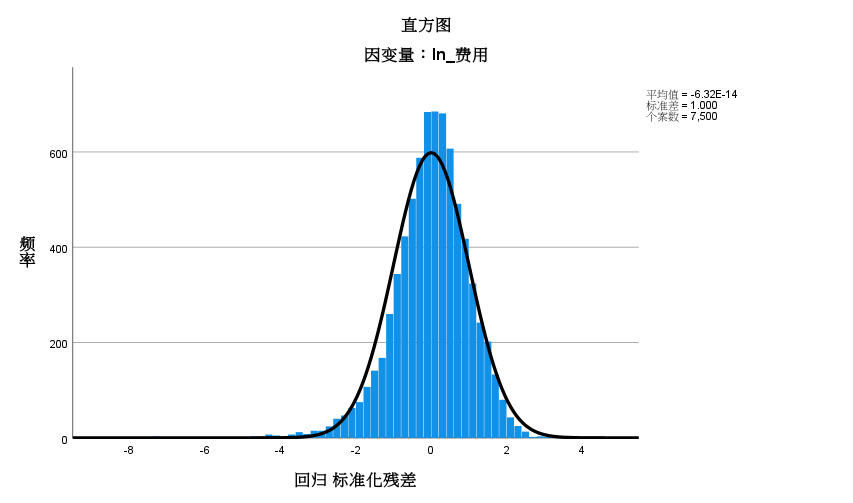
\includegraphics[width=0.8\textwidth]{回归模型标准化残差直方图.png}
\caption{回归模型标准化残差直方图}
\label{fig:hist_res}
\end{figure}

\begin{figure}[H]
\centering
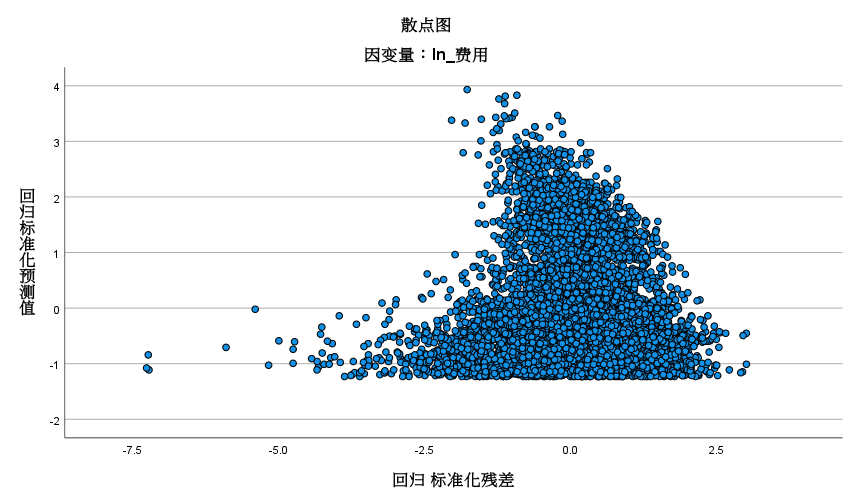
\includegraphics[width=0.8\textwidth]{最终回归模型标准化残差散点图.png}
\caption{最终回归模型标准化残差散点图}
\label{fig:scatter_res}
\end{figure}

\subsection{主成分分析（PCA）}

\subsubsection{主成分分析适用性检验}

为进一步挖掘影响医疗支出的核心维度，对纳入回归的11个自变量开展主成分分析。在进行主成分提取之前，首先通过KMO检验和Bartlett球形检验判断数据是否适合进行因子分析，结果如表~\ref{tab:pca_kmo}所示。

\begin{table}[H]
\centering
\caption{KMO和Bartlett球形检验结果}
\label{tab:pca_kmo}
\begin{tabular}{c c c}
\toprule
检验方法 & 统计量 & 数值 \\
\midrule
KMO取样适切性量数 & — & 0.514 \\
\cmidrule{2-3}
\multirow{3}{*}{Bartlett球形检验} & 近似卡方 & 17697.394 \\
& 自由度 & 55 \\
& 显著性 & 0.000 \\
\bottomrule
\end{tabular}
\end{table}

KMO值为0.514，大于0.5的最低可接受阈值，表明变量间存在一定的共同因素，基本适合进行主成分分析；Bartlett球形检验的p值小于0.001，拒绝变量间相互独立的原假设，进一步证实了数据适合进行降维处理。

\subsubsection{主成分提取与结果分析}

采用方差最大正交旋转法提取公共因子，SPSS输出结果如表~\ref{tab:pca_eigen}、表~\ref{tab:pca_load}所示。

表~\ref{tab:pca_eigen}为主成分分析的总方差解释结果。根据特征值大于1的提取准则，共提取5个主成分，累计方差贡献率达67.00\%，能够解释原始变量超过三分之二的变异信息，在有效保留核心数据特征的同时实现了变量降维。

\begin{table}[H]
\centering
\caption{主成分分析总方差解释结果}
\label{tab:pca_eigen}
\begin{tabular}{cccc}
\toprule
主成分 & 特征值 & 方差贡献率（\%） & 累计方差贡献率（\%） \\
\midrule
1 & 2.459 & 22.356 & 22.356 \\
2 & 1.772 & 16.108 & 38.464 \\
3 & 1.123 & 10.211 & 48.675 \\
4 & 1.015 & 9.228 & 57.903 \\
5 & 1.001 & 9.098 & 67.001 \\
\bottomrule
\multicolumn{4}{l}{\textit{注：仅列出特征值大于$1$的$5$个主成分，其余主成分特征值均小于$1$。}}
\end{tabular}
\end{table}

表~\ref{tab:pca_load}为方差最大正交旋转后的主成分载荷矩阵，结合载荷绝对值较高的变量含义，对各主成分进行命名与解读如下：
\begin{enumerate}[(1)]
\item 主成分1：在压力水平、睡眠时长、慢性病数量、去年住院次数上具有较高载荷，反映了心理压力、睡眠质量与躯体健康状况、医疗利用程度的内在关联，可命名为\textbf{身心健康状况维度}，是影响医疗支出的核心维度。
\item 主成分2：在胆固醇、年龄上载荷极高，同时与身体质量指数正相关，体现了年龄增长伴随的生理指标变化特征，可命名为\textbf{年龄与生理指标维度}。
\item 主成分3：在年就诊次数、吸烟者编码上载荷较高，且与慢性病数量正相关，反映了医疗服务利用程度与健康行为的关联。值得注意的是，吸烟者编码在该主成分上为负载荷（-0.626），提示吸烟行为与医疗服务利用呈反向关联，可能反映了吸烟者因健康问题更倾向于住院治疗而非门诊就诊的行为模式，可命名为\textbf{医疗服务利用维度}。
\item 主成分4：在\(\ln\)\_收入、身体质量指数上载荷较高，反映了个体社会经济水平与身体形态特征，可命名为\textbf{收入与体质维度}。
\item 主成分5：在周饮酒量上载荷极高，主要反映个体的饮酒行为习惯，可命名为\textbf{饮酒行为维度}。
\end{enumerate}

\begin{table}[H]
\centering
\caption{旋转后主成分载荷矩阵}
\label{tab:pca_load}
\begin{tabular}{cccccc}
\toprule
变量 & 主成分1 & 主成分2 & 主成分3 & 主成分4 & 主成分5 \\
\midrule
压力水平 & 0.909 & — & — & — & — \\
睡眠时长 & -0.774 & — & — & — & — \\
慢性病数量 & 0.625 & — & 0.497 & — & — \\
去年住院次数 & 0.622 & — & — & — & — \\
胆固醇 & — & 0.913 & — & — & — \\
年龄 & — & 0.842 & — & — & — \\
年就诊次数 & — & — & 0.677 & — & — \\
吸烟者编码 & 0.346 & — & -0.626 & — & — \\
\(\ln\)\_收入 & — & — & — & 0.769 & — \\
身体质量指数 & — & 0.315 & — & 0.611 & 0.338 \\
周饮酒量 & — & — & — & — & 0.882 \\
\bottomrule
\multicolumn{6}{l}{\textit{注：载荷绝对值小于$0.3$的结果以“—”标注，采用方差最大正交旋转法。}}
\end{tabular}
\end{table}

主成分分析结果将11个原始影响因素归纳为5个核心维度，与前文多元线性回归的结论高度呼应，进一步明确了身心健康状况、医疗服务利用是驱动医疗支出的核心方向，为后续医保政策优化与人群健康管理措施制定提供了更聚焦的理论依据。

\section{结论与建议}

\subsection{研究结论分析}

根据上述基于SPSS的全流程统计分析结果，可以得出以下核心结论：

\begin{enumerate}[label=(\arabic*)]
\item \textbf{健康行为是影响医疗支出的第一核心因素}。吸烟行为对医疗支出的正向影响最大，吸烟者的年医疗费用比非吸烟者平均高出12987美元，在控制其他变量后，吸烟者的医疗支出约为非吸烟者的2.02倍。这一发现与国外相关研究结论高度一致，表明吸烟是驱动医疗费用增长的首要可控风险因素。

\item \textbf{健康状况与医疗利用是影响医疗支出的第二核心因素}。慢性病数量每增加一种，年医疗费用上升约17.7\%；年就诊次数、住院次数与医疗支出呈显著正相关，医疗利用行为的增加直接推动费用上涨。同时，年龄每增长1岁，医疗支出上升约0.6\%，年龄增长伴随的器官功能衰退与多病共存，是医疗费用增长的重要驱动因素。

\item \textbf{社会经济与人口学特征的影响相对有限}。BMI、年收入与医疗支出呈显著正相关，但边际效应较小；性别和地区差异对医疗支出的影响不显著，运动水平在回归中表现为显著负向影响，说明控制健康行为与健康状况后，这些因素的解释力有所不同。

\item \textbf{模型拟合效果与稳健性良好}。最终的多元线性回归模型调整R²为0.684，整体解释力较好，模型的F检验、t检验、残差诊断及异方差检验均符合经典假设，估计结果稳健可靠。主成分分析进一步验证了健康行为、健康状况是影响医疗支出的两大核心维度，与回归结论高度一致。
\end{enumerate}

从实际机理上分析，吸烟导致呼吸系统疾病、心血管疾病及多种癌症的风险显著增加，对应的诊疗费用、住院费用及长期用药费用均大幅上升。慢性病（如高血压、糖尿病、慢阻肺）需要持续管理，定期复诊和药物费用的累积效应明显。年龄增长伴随器官功能衰退，多病共存概率增加，因此费用随年龄单调递增。上述结论符合医学常识和经济学直觉，实证结论基本正确。

\subsection{对策建议}

基于本文的研究结论，从健康干预、医保政策及资源配置角度提出以下四项建议，以控制医疗费用不合理增长，保障医保基金的可持续性。

\subsubsection{强化控烟干预，抑制吸烟相关医疗支出}

鉴于吸烟行为的边际影响最大，应将控烟作为降低医疗支出的首要公共卫生策略。建议：
\begin{enumerate}[label=(\arabic*)]
\item 提高烟草税和香烟零售价，利用价格杠杆减少吸烟率，同时将烟草税收入专项用于医保基金补贴和控烟宣传。
\item 将戒烟药物和戒烟咨询纳入医保报销范围，降低吸烟者戒烟的经济障碍，同时在基层医疗机构推广标准化戒烟门诊服务。
\item 在公共场所全面禁烟，加强对未成年人吸烟的管控，通过媒体宣传、社区教育等方式，普及吸烟危害，形成全社会控烟的良好氛围。
\end{enumerate}
据本文研究结果估算，每帮助一名吸烟者成功戒烟，未来年均可节省医疗支出约12987美元，控烟干预的成本收益比极高。

\subsubsection{推进慢性病分级管理，控制疾病进展与费用增长}

慢性病数量每增加一种，费用上升约17.7\%，提示慢病预防和早期干预是控制医疗费用的关键环节。建议：
\begin{enumerate}[label=(\arabic*)]
\item 全面推广家庭医生签约服务，对高血压、糖尿病等常见慢病患者实施定期随访、用药指导和健康管理，建立“预防-诊疗-康复”全周期服务链条。
\item 建立基于电子健康档案的慢病风险预警系统，对高危人群提前开展健康干预，通过饮食指导、运动干预等方式，降低慢病发病率，延缓疾病进展。
\item 改革医保支付方式，对慢病患者实行“按人头付费+健康管理包”的支付模式，将医保基金支出与患者健康结果挂钩，激励基层医疗机构主动做好慢病管理，降低患者的住院率和并发症发生率。
\end{enumerate}

\subsubsection{优化医疗资源配置，减少不必要的医疗利用}

就诊次数、住院次数与医疗支出呈显著正相关，减少非必要的医疗利用是控制费用的重要途径。建议：
\begin{enumerate}[label=(\arabic*)]
\item 严格落实基层首诊和分级诊疗制度，明确各级医疗机构的诊疗范围，引导轻症患者在社区医疗机构解决，减少三级医院的非必要门诊就诊，优化医疗资源配置效率。
\item 大力推广互联网复诊、远程医疗和线上健康咨询服务，为慢病患者、轻症患者提供便捷的线上诊疗服务，减少非必要的线下门诊就诊，降低患者的就医成本和医保基金支出。
\item 对频繁就诊、反复住院的患者进行健康评估，识别潜在的身心健康问题，提供整合式照护服务，避免重复检查、重复诊疗，减少医疗资源的浪费。
\end{enumerate}

\subsubsection{完善医保差异化支付政策，建立健康激励机制}

针对吸烟者、多慢病患者等高费用人群，应探索建立差异化的医保支付政策，引导参保人主动改善健康行为。建议：
\begin{enumerate}[label=(\arabic*)]
\item 建立医保与健康管理的联动机制，对参加健康管理计划并达到控烟、减重、规律服药、定期体检等健康目标的参保人，降低其个人自付比例或返还部分医保保费，激励参保人主动改善健康行为。
\item 设置差异化的医保起付线和共付比例，对吸烟、酗酒等不健康行为导致的疾病，适当提高个人自付比例；对通过健康管理有效控制慢病的患者，适当降低自付比例，体现医保政策的正向激励导向。
\item 针对高风险人群开展精准化的医保干预，对吸烟者、多慢病患者等，提供免费的健康管理服务和疾病预防服务，从源头降低疾病发生风险，减少未来的医保基金支出。
\end{enumerate}

\subsection{研究局限与展望}

本研究虽取得了一定发现，但仍存在以下局限性，有待未来研究进一步完善：

\begin{enumerate}[label=(\arabic*)]
\item \textbf{数据来源的局限性}：本文使用的数据为美国医疗保险数据，其医疗体系、定价机制、保险制度与我国存在较大差异，研究结论在直接推广至中国情境时需保持审慎。未来研究可采用中国本土数据（如CHNS、CHARLS等）进行对比分析。

\item \textbf{因果识别的局限性}：本研究基于横截面数据，采用多元线性回归方法只能揭示变量间的统计关联，难以严格识别因果关系。例如，医疗利用（就诊次数、住院次数）与医疗支出之间可能存在反向因果或遗漏变量偏误。未来可尝试采用面板数据、工具变量法或双重差分法等准实验方法，进一步探究因果关系。

\item \textbf{变量控制的不足}：尽管本文纳入了较为丰富的健康行为和医疗利用变量，但仍可能遗漏了如医保报销比例、自付额度、医疗服务价格、家庭支持等制度性与社会性因素，这些变量可能对个人医疗支出产生重要影响。

\item \textbf{模型非线性的探索}：本文主要采用线性回归模型，未能充分捕捉变量之间可能存在的非线性关系（如年龄与费用的非线性、吸烟与慢病的交互效应等）。未来可引入机器学习方法（如随机森林、梯度提升树）或非线性回归模型，更灵活地刻画医疗支出的复杂决定机制。
\end{enumerate}

综上所述，本文基于SPSS 27.0软件，利用7500条医疗保险个人数据，通过描述性统计、均值差异检验、相关性分析、多元线性回归、主成分分析等多种方法，系统剖析了医疗保险个人支出的影响因素，识别出吸烟、慢性病数量和年龄是三大核心影响因素。研究结论可为我国医保基金精细化管理、健康干预政策制定及商业健康险产品设计提供量化参考。


\newpage
\addcontentsline{toc}{section}{参考文献}

\section*{\makebox[\textwidth][c]{参考文献}}

\nocite{*}
\printbibliography

\end{document}